\documentclass[11pt]{article}

\usepackage[margin=1in]{geometry}
\usepackage[T1]{fontenc}
\usepackage[utf8]{inputenc}
\usepackage{amsmath,amssymb}
\usepackage{graphicx}
\usepackage{booktabs}
\usepackage{xcolor}
\usepackage[round]{natbib}
\usepackage{hyperref}
\usepackage{caption}
\usepackage{authblk}
\usepackage{enumitem}
\usepackage{float}

\hypersetup{
  colorlinks=true,
  linkcolor=blue!50!black,
  citecolor=blue!50!black,
  urlcolor=blue!50!black
}

\title{\textbf{Clustered Memory Augmentation for Transformers:\\
A Bounded-Capacity Alternative to Raw Token Retention}}

\author[1]{[Author Name --- please insert before submission]}
\affil[1]{[Affiliation --- please insert before submission]}
\date{\today}

\begin{document}
\maketitle

\begingroup
\renewcommand{\thefootnote}{\fnsymbol{footnote}}
\footnotetext[1]{\textbf{AI-assistance disclosure.} The method design, reference implementation,
experiments, and the first draft of this manuscript were produced with substantial assistance
from Claude (Anthropic), an AI system, working under the direction of the listed author. All
reported numbers come from logged experiment runs (see supplementary code and
\texttt{results/raw\_results.jsonl}); none were invented or hand-adjusted after the fact.
The author is responsible for reviewing and vouching for the content before any submission,
and should disclose AI assistance per the policies of the venue this is submitted to.}
\endgroup

\begin{abstract}
Clustering is used throughout the efficient-Transformer literature to sparsify attention within
a fixed context or to compress an already-collected key/value cache offline, but --- in the prior
work we found --- not to maintain a persistent, hard-capacity-bounded memory across an unbounded
stream that must merge similar history and evict it online. We synthesize Clustered Memory
Augmentation (CMA), combining DP-means-style dynamic cluster creation with VQ-VAE-style EMA
updates and stop-gradient training inside a memory-augmented Transformer block, and release a
unit-tested reference PyTorch implementation. We then test a narrow question on a small,
CPU-only synthetic long-range recall task: at equal memory budget, does clustering organize
memory better than retaining the raw highest-scoring tokens (an H2O-style baseline)? At our
primary, tight budget (3 seeds), neither clustered nor raw-token memory separates from a
no-memory baseline, while a full-attention oracle does; this null result persists exactly, to the
precision of our evaluation set, across a further single-seed sweep to a $4\times$ larger budget.
We rule out the simplest explanation --- the memory branch learning to ignore retrieved content
entirely --- by direct measurement of its attention weights. Our next explanation --- that a
retrieval-selection query pooled once per processing chunk could not distinguish the multiple
queries our task places inside a single chunk --- turned out to be wrong: re-reading our own
retrieval code showed the reported configuration had already made candidate selection
query-independent for an unrelated reason, so pooled versus per-token selection could not have
mattered. We implement, unit-test, and rerun the full comparison under a corrected mechanism with
genuinely per-token, query-conditioned retrieval selection, and obtain the same null result again:
CMA still does not separate from the raw-token baseline. Wondering whether task difficulty itself
was the confound, we then substantially simplify the task while deliberately preserving pure
content-matching semantics (no recency or overwrite structure, which would let a simpler
heuristic solve it); the full-attention oracle's accuracy nearly doubles (from $0.336$ to
$0.669$), confirming the easier task is both learnable and meaningfully easier within the same
step budget, yet CMA and TopKRaw remain pinned to chance and, if anything, CMA trails TopKRaw
rather than leading it. Three specific candidate explanations for the null result --- collapse to
a null fallback slot, vacuous query-independent retrieval selection, and task difficulty --- are
thereby ruled out by direct measurement rather than by assumption, across three independently
reasoned rounds of experiments. We report this full self-correcting process and contribute the
synthesized method, the tested implementation, and the exclusion chain itself as this paper's
result: the remaining untested hypothesis --- that the memory cross-attention's own
content-matching circuit needs substantially more training than we gave it to bootstrap at all
--- is a question about training dynamics rather than about clustering versus raw retention, and
we treat stopping here, with three specific explanations ruled out rather than an unexplained
null, as a deliberate conclusion rather than an unfinished lead.
\end{abstract}

\section{Introduction}

Transformer self-attention costs $O(T^2)$ compute and its key/value (KV) cache costs $O(T)$
memory in the sequence length $T$. Long documents, long conversations, and long-running agents
routinely need $T$ far beyond what full attention or an unbounded KV cache can support, which has
motivated a large body of work on efficient attention and external memory (see
\citet{survey2025} for a broader survey than we attempt here).

Clustering recurs throughout this literature but, to our knowledge, has not been pushed all the
way to its logical conclusion as a memory-organization principle. It is used to sparsify
attention within a fixed context (Routing Transformer, Reformer, Cluster-Former;
Section~\ref{sec:related}), and it is used to compress an already-collected KV cache once, offline,
after a prompt is complete (ClusterAttn). What we did not find in our search is a method that
uses clustering to maintain a \emph{persistent, hard-capacity-bounded} memory across an
\emph{unbounded} stream --- one that must decide, online, when to merge semantically similar
history and when to evict it, so that memory size never grows past a fixed budget regardless of
how long the stream runs.

This paper makes three contributions, of clearly different character, which we do not want to
conflate:
\begin{enumerate}[leftmargin=1.4em,itemsep=1pt]
\item A synthesis, Clustered Memory Augmentation (CMA), that combines techniques from clustering
(DP-means-style dynamic cluster creation), generative modeling (VQ-VAE-style EMA codebook
updates and stop-gradient training), and the memory-augmented Transformer literature (EM-LLM's
dual-buffer retrieval, ClusterAttn's importance-based exemplar selection) into a single bounded
memory module (Section~\ref{sec:method}). Table~\ref{tab:provenance} states plainly which parts
are adaptations of a specific prior method and which parts are our own combination.
\item A reference PyTorch implementation, independently unit-tested for correctness of the
data structures and gradient flow (9/9 tests passing across two test suites, including tests added
partway through this study to validate the corrected retrieval mechanism of
Section~\ref{sec:results-diagnosis} before trusting it in a training run; see the supplementary
code), decoupled from the question of whether the method is empirically useful.
\item A small, honest empirical test on a synthetic long-range recall task, comparing CMA against
a matched-budget raw-token-retention baseline, a no-memory lower bound, and a full-attention
upper bound (Sections~\ref{sec:setup}--\ref{sec:results}). We report what we found, including a
failed initial configuration (Section~\ref{sec:calibration}) and, once the task was learnable at
all, a null result at every budget we tried: neither bounded-memory method separates from the
no-memory baseline or from each other. We then instrument the model directly, rule out the
simplest explanation (collapse to a null fallback), propose a second explanation (a chunk-pooled
retrieval query), discover by re-reading our own code that this second explanation cannot be right
in our configuration, and implement, unit-test, and rerun the full comparison under a corrected,
genuinely query-conditioned retrieval mechanism --- which reproduces the same null result
(Section~\ref{sec:results-diagnosis}). We report this self-correction in the open rather than
quietly replacing the first explanation with the second. Suspecting task difficulty itself might
be a third confound, we then rerun the comparison on a substantially easier version of the same
content-matching task --- fewer pairs, a smaller vocabulary, a wider gap between writing and
querying, but deliberately no recency or overwrite structure that would let a simpler heuristic
solve it --- and obtain the same null result a third time, even though a full-attention oracle's
accuracy on this easier task nearly doubles (Section~\ref{sec:results-easytask}), ruling out
difficulty as well. We report the full three-round exclusion chain, together with the ways our
compute budget (a 2-core CPU machine, no GPU) limits the scale and statistical power of the whole
comparison (Section~\ref{sec:limitations}).
\end{enumerate}

We want to be explicit about scope. This is not a claim that CMA is state-of-the-art, nor that it
has been validated on real language modeling; it is a controlled small-scale test of one specific
question --- \emph{at equal memory budget, does organizing memory by clustering beat simply
keeping the highest-scoring raw tokens?} --- together with a fully worked reference
implementation. As reported in Section~\ref{sec:results}, our own test of that question did not
resolve it, across three rounds: our first diagnosis of why turned out to be wrong, our corrected,
properly-tested follow-up experiment produced the same null result as the original, and a third
round that specifically isolated task difficulty as a possible confound produced the same null
result again despite the task itself becoming demonstrably easier. We offer the method, the
implementation, and all three diagnostic rounds (including the one that was wrong, left visible
rather than deleted) so that the original question can be tested again, by us or by others, if the
leading remaining hypothesis --- that the memory cross-attention's content-matching circuit itself
needs substantially more training than we gave it to bootstrap at all --- is ever tested directly.
We did not pursue that test ourselves; Section~\ref{sec:limitations} explains why we treat that as
a deliberate stopping point for this paper rather than a resource shortfall.

\section{Related Work}
\label{sec:related}

We group prior work by the mechanism used to control the cost of attending to, or storing,
long historical context.

\paragraph{Clustering-based sparse attention.}
Routing Transformer~\citep{roy2021routing} clusters queries and keys with online mini-batch
$k$-means and restricts attention to tokens in the same cluster, reducing complexity from
$O(T^2)$ to roughly $O(T^{1.5})$; cluster centroids are updated with an exponential moving
average (EMA) during training. Reformer~\citep{kitaev2020reformer} replaces explicit clustering
with locality-sensitive hashing (LSH), bucketing similar queries/keys without an iterative
clustering objective. Cluster-Former~\citep{wang2020clusterformer} combines sliding-window local
attention with cross-window clustering attention to recover long-range dependencies that pure
local attention misses. Most relevant to our design choices, Mixture of Sparse
Attention~\citep{mosa2025} reports that Routing Transformer's token-level online $k$-means
``may fail to yield performance gains due to slow convergence,'' and replaces it with
expert-choice routing; we treat this as evidence that token-level, unconstrained online
clustering is not obviously stable, and we deliberately cluster at a coarser (segment)
granularity instead (Section~\ref{sec:method}).

\paragraph{External memory and retrieval augmentation.}
Memorizing Transformers~\citep{wu2022memorizing} maintain a non-differentiable cache of past
key/value pairs and retrieve approximate nearest neighbors for local attention. kNN-LM
~\citep{khandelwal2020knnlm} interpolates a language model's output distribution with a
non-parametric nearest-neighbor distribution over a datastore. Product-key
memory~\citep{lample2019memory} and its large-scale successor, Memory Layers at
Scale~\citep{meta2024memorylayers}, use a Cartesian-product key decomposition for sub-linear
lookup into memory layers with up to $10^{11}$ parameters, at negligible extra FLOPs.

\paragraph{Hierarchical and compressive memory.}
Transformer-XL~\citep{dai2019transformerxl} caches the previous segment's hidden states for
segment-level recurrence. The Compressive Transformer~\citep{rae2020compressive} adds a
secondary compressed memory: hidden states evicted from the primary cache are compressed
(rather than discarded) into a larger, lower-fidelity store. HMT~\citep{he2025hmt} organizes
memory into sensory/short-term/long-term tiers with cross-attention retrieval as a
model-agnostic plug-in, but uses fixed-length segmentation rather than clustering.

\paragraph{Clustering-based KV-cache compression at inference time.}
H2O~\citep{zhang2023h2o} retains ``heavy-hitter'' tokens with the highest cumulative attention
mass plus recent tokens. StreamingLLM~\citep{xiao2024streaming} shows that keeping a handful of
initial ``attention sink'' tokens plus a sliding window suffices for stable generation far
beyond the training length, without retraining; we borrow the underlying intuition for the
learned null slot in our cross-attention (Section~\ref{sec:method}). Most directly related to
this paper, ClusterAttn~\citep{clusterattn2025} observes that individual attention heads
consistently attend to a small number of token clusters within a prompt, and uses a
DBSCAN-inspired density clustering algorithm to compress the KV cache accordingly, reporting
10--65\% memory reduction and 2.6--4.8$\times$ throughput improvement at near-lossless accuracy.
ClusterAttn's clustering, however, runs once, offline, after the full prompt is available, and
is designed for compressing an already-materialized cache rather than for maintaining a bounded
memory across an unbounded stream.

\paragraph{Event-driven online clustering memory.}
EM-LLM~\citep{emllm2025} detects event boundaries with a Bayesian-surprise signal and refines
them with graph modularity optimization over a local window --- in effect, an online clustering
procedure --- then retrieves with a two-buffer scheme combining content similarity and temporal
contiguity, scaling to $10^{7}$-token contexts. Titans~\citep{titans2025} instead triggers a
parametric associative memory update via a KL-divergence surprise signal, learned as a
test-time optimization problem. Our Section~\ref{sec:method} borrows EM-LLM's segmentation and
dual-buffer retrieval ideas most directly.

\paragraph{Summary.} As of our search (Section~\ref{sec:related} reflects a literature search
conducted in July 2026 and is not a systematic review), clustering is well established either
as an attention-sparsification tool (Routing Transformer, Reformer, Cluster-Former) or as an
offline KV-cache compression tool (ClusterAttn), but we did not find prior work combining
clustering with a \emph{hard, persistent capacity bound} that supports merging and eviction over
an unbounded stream --- the specific combination this paper explores. We say more about which
parts of our design are direct adaptations versus new combinations in
Section~\ref{sec:method-summary}.

\section{Method: Clustered Memory Augmentation}
\label{sec:method}

Clustered Memory Augmentation (CMA) maintains, per stream, a memory of at most $K_{\max}$
\emph{clusters}. Each cluster stores a centroid (a soft summary used only for retrieval
similarity) and up to $E$ raw \emph{exemplar} tokens (hard samples used to reconstruct detail).
The design has six components, M1--M6, which we describe in turn; Table~\ref{tab:provenance}
in Section~\ref{sec:method-summary} states explicitly which parts are adapted from a specific
prior method versus assembled by us.

\paragraph{M1: segment boundary detection.}
Rather than clustering individual tokens --- which Section~\ref{sec:related} noted is a source
of instability in Routing Transformer --- we first group tokens into coarser segments. Following
EM-LLM's Bayesian-surprise segmentation, we track a proxy surprise signal (one minus the cosine
similarity between consecutive token hidden states, replacing EM-LLM's language-model
negative log-likelihood so the module does not depend on a specific LM head) and flag a new
segment whenever this signal exceeds a running mean plus $\gamma$ standard deviations over a
sliding window. In our experiments (Section~\ref{sec:setup}) we use fixed-length chunks instead,
for simplicity and to match the chunked processing of the baselines; the boundary detector is
implemented and unit-tested but not used in the reported experiments (Section~\ref{sec:limitations}).

\paragraph{M2: bounded online clustering.}
Each segment is pooled (mean pooling in our implementation) into a representation vector and
compared by cosine similarity to existing active cluster centroids. If the best match exceeds a
merge threshold $\tau$, the segment is absorbed into that cluster: the centroid is updated by
EMA, mirroring how VQ-VAE~\citep{vqvae2017} updates codebook vectors and avoiding the
per-step gradient updates that make online $k$-means noisy. If no cluster matches, a new one is
created --- this create-or-merge rule is exactly DP-means~\citep{dpmeans2012}, the
small-variance asymptotic limit of a Dirichlet-process Gaussian mixture, which lets the number
of clusters grow with the data instead of being fixed in advance as in classical $k$-means.
Because the stream is unbounded, cluster count is capped at $K_{\max}$: when a new cluster is
needed and none of the $K_{\max}$ slots is free, we first reclaim any ``dead'' cluster (unused
for longer than a TTL), and otherwise merge the two most similar active clusters (a
count-weighted linear combination of centroids, renormalized --- a cheap approximation to a
spherical mean) to free a slot, echoing the Compressive Transformer's ``compress rather than
discard'' treatment of aging memory, but applied to whole clusters instead of individual states.
For end-to-end training, cluster assignment can optionally be treated as vector quantization:
a straight-through estimator lets gradients skip the non-differentiable nearest-centroid lookup,
with an optional VQ-VAE-style commitment loss. Our reported experiments do not use this path
(Section~\ref{sec:setup}); the memory write is a stop-gradient operation, matching how
Memorizing Transformers and EM-LLM also treat their memories as non-differentiable.

\paragraph{M3: hybrid compressed representation.}
Keeping only centroids loses detail (the standard weakness of compression functions such as the
Compressive Transformer's); keeping every raw token loses the compression benefit entirely (as
in Memorizing Transformers). CMA keeps both: a centroid for cheap similarity search, and the
$E$ highest-scoring raw exemplar tokens per cluster, ranked by an importance proxy (we use
hidden-state $\ell_2$ norm; ClusterAttn and H2O suggest cumulative attention mass as a
higher-fidelity alternative when available). When two clusters merge, their exemplar sets are
unioned and truncated back to $E$ by score, so a merge can never silently drop the single most
important token of either parent cluster.

\paragraph{M4: retrieval.}
A query is pooled into a vector and compared to all active centroids; the top-$k_{\text{sim}}$
most similar clusters are retrieved, together with the $k_{\text{recent}}$ most recently written
clusters regardless of similarity --- a direct adaptation of EM-LLM's similarity-buffer plus
contiguity-buffer retrieval. The selected clusters' exemplar tokens are concatenated and used as
keys/values for a cross-attention layer, along with one learned ``null'' slot that is always
unmasked; the null slot guarantees a valid softmax even when memory is empty (e.g., at the start
of a stream) and is motivated by the attention-sink phenomenon reported for
StreamingLLM. When $K_{\max}$ is large, the $O(K_{\max})$ linear scan over centroids can be
replaced by the product-key decomposition of Memory Layers at Scale to reach
$O(\sqrt{K_{\max}})$; our implementation provides the simpler $O(K_{\max})$ version.

\paragraph{M5: eviction policy.}
Beyond the merge-on-capacity rule in M2, we implement two alternative eviction policies: plain
least-recently-used, and a frequency$\times$recency-decay score reminiscent of H2O's
heavy-hitter criterion, applied to clusters rather than individual tokens.

\paragraph{M6: integration.}
CMA is designed as a plug-in cross-attention layer that can be inserted into a pretrained
Transformer without modifying the backbone, following HMT's model-agnostic positioning; the
backbone can be frozen (lightweight adapter-style training of only the new layer) or fine-tuned
jointly.

\subsection{Provenance: what is adapted versus new}
\label{sec:method-summary}

\begin{table}[H]
\centering
\small
\begin{tabular}{p{2.1cm}p{4.6cm}p{4.9cm}}
\toprule
\textbf{Module} & \textbf{Primary source(s)} & \textbf{What is new here} \\
\midrule
M1 & EM-LLM (simplified: no graph-modularity refinement) & Decoupled from a specific LM head \\
M2 & DP-means (create-or-merge rule) + VQ-VAE (EMA update, stop-gradient, dead-code reset) & Combining a nonparametric-clustering rule with a generative-model quantization training
recipe for \emph{bounded, mergeable} online memory; we did not find this specific combination
in our search \\
M3 & Retrieval framing from Memorizing Transformers; exemplar scoring from ClusterAttn/H2O & The
merge-time union-then-truncate rule for exemplars, to bound information loss under merging \\
M4 & EM-LLM (dual-buffer retrieval); StreamingLLM (motivates the null slot); optional speed-up
from Memory Layers at Scale & Retrieval target is a cluster rather than a token or event \\
M5 & H2O (importance scoring, adapted to clusters) & --- \\
M6 & HMT (model-agnostic plug-in) & --- \\
\bottomrule
\end{tabular}
\caption{Provenance of each module. We flag M2 as the main place where we combined techniques
from different subfields (nonparametric clustering and generative-model vector quantization)
rather than adapting a single prior system; absence of a cited exact match reflects the scope of
our literature search (Section~\ref{sec:related}), not a strong novelty claim.}
\label{tab:provenance}
\end{table}

\section{Experimental Setup}
\label{sec:setup}

We evaluate on a synthetic long-range associative recall task in the style of the
multi-query associative recall (MQAR) diagnostics used to study efficient sequence
architectures~\citep{arora2024zoology}, rather than a real pretrained language model: our
environment has no GPU (2 CPU cores only), so a real-LM evaluation at a scale that would be
informative is not feasible in reasonable time. We designed the smallest task we believe still
tests the mechanism honestly, and report exactly what it shows, including where results are
weak or inconclusive.

\subsection{Task}
Each sequence of length $T{=}192$ embeds $P{=}4$ key--value pairs (keys and values drawn from
disjoint 16-symbol vocabularies) at random, mutually non-overlapping positions within the first
60\% of the sequence, with every other position filled by an i.i.d.\ random filler token from a
separate 32-symbol vocabulary; each pair is constrained to fall inside a single processing chunk
(Section~\ref{sec:setup}, chunk size 32) so a chunk-local model can in principle see a key and
its value together. The final 12 positions present the $P$ keys again, in random order, each as
an explicit \texttt{(QUERY, key, value)} triple; loss and accuracy are computed only at the
position immediately after each queried key, i.e., the model must predict the paired value
having seen the key but not (due to the causal mask) the value that follows it in the tensor.
Because the value is written explicitly at training time, this is a standard teacher-forced
next-token setup restricted to the positions we care about, not a departure from ordinary
language-model training. All pairs are placed at least $\sim$75 positions before the query
block, more than twice the 32-token chunk size, so a model restricted to local attention
provably cannot solve the task from the local window alone.

\subsection{Conditions}
All four conditions share the same token embedding table, RoPE-based causal self-attention
implementation, feed-forward width, and output head; they differ only in what --- if anything ---
is added on top of chunk-local self-attention.
\begin{itemize}[leftmargin=1.4em,itemsep=1pt]
\item \textbf{NoMemory}: chunk-local causal self-attention only (window $=$ chunk size $=32$);
a lower bound that should stay near chance, since no pair is ever visible from the query chunk.
\item \textbf{FullAttn}: standard causal self-attention over the entire 192-token sequence, no
chunking; an upper-bound oracle with unrestricted access to the whole context.
\item \textbf{TopKRaw}: NoMemory plus a fixed-capacity raw-token memory (an H2O-style baseline):
the $B$ individually highest-scoring tokens seen so far (by the same importance proxy CMA uses)
are retained verbatim; no clustering or compression.
\item \textbf{CMA}: NoMemory plus the clustered memory of Section~\ref{sec:method}, with
$E{=}2$ exemplars per cluster (matched to the pair length) and $K_{\max} = B/2$ clusters, so
that TopKRaw and CMA always hold the same total number of token-sized memory slots $B$.
\end{itemize}
TopKRaw and CMA reuse the identical \texttt{ClusteredMemoryCrossAttention} module (same
parameters, same code path) from our reference implementation, differing only in the memory
bank object underneath; this is what makes the comparison isolate ``clustering versus flat
top-$B$ retention'' rather than conflating it with unrelated implementation differences. Both
retrieve their entire budget every step ($k_{\text{sim}} = K_{\max}$, $k_{\text{recent}}=0$:
recency carries no signal in this task since all pairs are inserted in a single early burst),
so the comparison is specifically about how memory content is organized under a shared budget
and a shared retrieval mechanism, not about retrieval selection.

\subsection{Matched-budget sweep}
Our primary comparison uses a deliberately tight budget $B{=}4$ --- half of the $P \cdot 2 = 8$
tokens that would be needed to store all four pairs verbatim --- so that some form of
compression or selection is required for either bounded-memory method to do well. We run this
primary comparison (all four conditions) with 3 random seeds. As a secondary, illustrative
sweep, we additionally run TopKRaw and CMA at $B \in \{8, 16\}$ with a single seed each, to show
the trend as budget increases toward and beyond the ``just enough'' point; we label these
single-seed results explicitly as lower-confidence in Section~\ref{sec:results}.

\subsection{Optimization}
All models use $d_{\text{model}}{=}64$, 2 layers, 4 attention heads, and RoPE positional
encoding rather than learned absolute position embeddings (see below). We train with Adam,
peak learning rate $3\times10^{-3}$ with 100-step linear warmup followed by cosine decay to
0 over 1300 steps, gradient-norm clipping at 1.0, batch size 16 (evaluation batch size 256,
freshly sampled and disjoint in random seed from the training stream). All hyperparameters were
fixed during a calibration phase (Section~\ref{sec:calibration}) and then \emph{not} tuned
per-condition or per-seed on the reported runs.

\subsection{A note on calibration and why we use RoPE}
\label{sec:calibration}
Recovering a value from an earlier position given only its key is, mechanistically, an
\emph{induction head}: interpretability work on small transformers~\citep{olsson2022induction}
shows this typically requires composing two attention layers (one to represent ``the previous
token,'' a second to match the current token against that representation elsewhere in context)
and is markedly easier to learn under position representations where ``attend one step back'' is
a single position-independent pattern, such as relative or rotary encodings, than under learned
absolute position embeddings, where the same pattern must be re-learned at every absolute
offset. Our first calibration pass used a single layer with learned absolute position
embeddings; \emph{all four conditions, including the FullAttn oracle, failed to learn at all}
and their evaluation loss plateaued exactly at $\log(16) \approx 2.77$, i.e., uniform-random
performance. Only after switching to two layers and RoPE did FullAttn begin to climb reliably
above chance. We report this failed configuration because it is informative: it shows that our
positive results below are not an artifact of an easy task, and that getting a synthetic
recall benchmark to be learnable at all is itself a nontrivial part of running this kind of
evaluation honestly.

\section{Results}
\label{sec:results}

We report the primary comparison first, then explain --- with direct supporting measurements,
not speculation --- why it does not separate the four conditions the way we expected, then report
the secondary budget sweep, which turns out to be consistent with that explanation.

\subsection{Primary comparison ($B{=}4$, 3 seeds)}
\label{sec:results-primary}

Table~\ref{tab:primary} and Figure~\ref{fig:primary-bar} show final evaluation accuracy for all
four conditions at the tight primary budget. FullAttn is the only condition that clearly
separates from chance ($1/16 = 0.0625$): its 3-seed mean of $0.336$ is roughly six times its own
3-seed standard deviation above chance ($0.336$ vs.\ $0.062 \pm 0.043$) --- a large gap even
allowing that 3 seeds cannot support a formal significance test --- indicating the task is
learnable in principle within our step budget. NoMemory, TopKRaw, and CMA all remain within about one standard deviation
of chance and of each other: NoMemory $0.067 \pm 0.010$, TopKRaw $0.077 \pm 0.009$, CMA
$0.072 \pm 0.005$ (mean $\pm$ std over 3 seeds; raw per-seed values in
Table~\ref{tab:primary-raw}). TopKRaw's mean is nominally the highest of the three and CMA's
standard deviation is nominally the tightest, but with 3 seeds and this much overlap in the raw
values, we do not read either as a real difference --- and we specifically do not want to
selectively report the metric (mean or std) that happens to favor CMA. Figure~\ref{fig:learning-curves}
shows the corresponding learning curves: FullAttn climbs steadily and has not plateaued by step
1300 (see Section~\ref{sec:limitations}); the other three conditions are flat and visually
overlapping for the entire run.

\begin{table}[H]
\centering
\small
\begin{tabular}{lrrrr}
\toprule
Condition & Params & Eval accuracy (mean $\pm$ std) & Eval loss (mean) & $n$ seeds \\
\midrule
NoMemory (lower bound) & 108{,}032 & $0.067 \pm 0.010$ & 2.774 & 3 \\
FullAttn (oracle) & 108{,}032 & $0.336 \pm 0.043$ & 2.028 & 3 \\
TopKRaw ($B{=}4$) & 141{,}184 & $0.077 \pm 0.009$ & 2.766 & 3 \\
CMA ($B{=}4$) & 141{,}184 & $0.072 \pm 0.005$ & 2.768 & 3 \\
\bottomrule
\end{tabular}
\caption{Primary comparison at the tight memory budget $B{=}4$, 3 random seeds. Chance-level
accuracy is $1/16=0.0625$; chance-level cross-entropy loss is $\ln 16 \approx 2.773$. Only
FullAttn separates clearly from chance.}
\label{tab:primary}
\end{table}

\begin{table}[H]
\centering
\small
\begin{tabular}{lccc}
\toprule
Condition & seed 0 & seed 1 & seed 2 \\
\midrule
NoMemory & 0.0674 & 0.0566 & 0.0762 \\
FullAttn & 0.3145 & 0.3086 & 0.3857 \\
TopKRaw ($B{=}4$) & 0.0674 & 0.0850 & 0.0781 \\
CMA ($B{=}4$) & 0.0674 & 0.0703 & 0.0771 \\
\bottomrule
\end{tabular}
\caption{Raw per-seed final evaluation accuracy underlying Table~\ref{tab:primary}, reported in
full since 3 seeds is too few for a mean/std summary to stand on its own.}
\label{tab:primary-raw}
\end{table}

\begin{figure}[H]
\centering
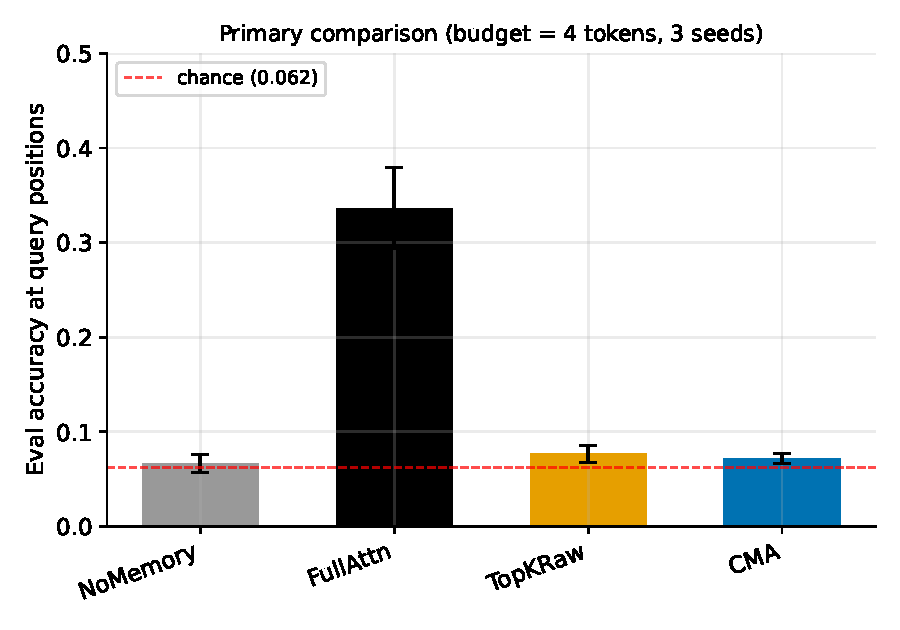
\includegraphics[width=0.62\linewidth]{figures/fig_primary_bar.pdf}
\caption{Primary comparison at $B{=}4$, 3-seed mean with standard-deviation error bars. Dashed
red line marks chance level.}
\label{fig:primary-bar}
\end{figure}

\begin{figure}[H]
\centering
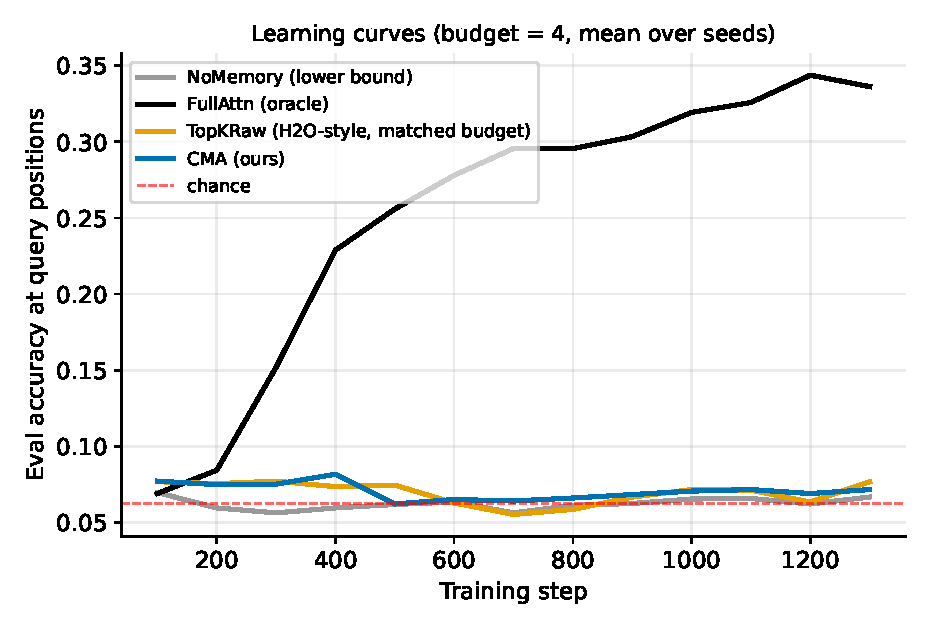
\includegraphics[width=0.72\linewidth]{figures/fig_learning_curves.pdf}
\caption{Learning curves at $B{=}4$, mean over 3 seeds. NoMemory, TopKRaw, and CMA overlap almost
entirely and stay flat at chance for the full 1300-step run; only FullAttn separates, and is still
rising at the end of training.}
\label{fig:learning-curves}
\end{figure}

\subsection{Why TopKRaw and CMA do not separate from chance: two ruled-out explanations and one
that survives}
\label{sec:results-diagnosis}

A comparison this flat is unsatisfying on its own --- it could mean clustering genuinely does not
help, or it could mean neither bounded-memory method ever learned to use its memory at all, which
would make the clustering-versus-raw-retention question moot rather than answered. Two
observations pointed us toward the second explanation, and we pursued both with supplementary
diagnostics (single seed, separate short runs, explicitly not part of the primary comparison
above).

\paragraph{Observation 1: TopKRaw and CMA track each other almost exactly, at every budget.}
At seed 0, TopKRaw and CMA's final evaluation accuracy is \emph{identical to the precision of our
evaluation set} ($0.0673828125$, i.e., exactly $69/1024$ correct) at every one of the three
budgets we tested, $B \in \{4, 8, 16\}$ (Table~\ref{tab:sweep} below), and matches NoMemory's
seed-0 run at most --- though, tellingly, not quite all --- of the thirteen evaluation checkpoints
during training. Two memory mechanisms that organize retained information completely differently
(verbatim tokens versus merged cluster centroids and exemplars) producing bit-identical downstream
accuracy across a $4\times$ budget range is not the pattern we would expect if either mechanism's
content were actually driving predictions.

\paragraph{Diagnostic A: the memory branch is not simply being ignored.} The most obvious
explanation for Observation 1 is that the memory cross-attention (Section~\ref{sec:method}, M4)
learns to route all of its softmax weight to the always-available learned null slot and none to
actually retrieved memory, in which case the specific memory content --- and therefore the budget
or the organization strategy --- would be irrelevant by construction. We instrumented the module
to record this weight directly and reran TopKRaw and CMA at $B{=}4$ for 700 steps (single seed,
otherwise identical recipe). Table~\ref{tab:null-attn} shows the mean null-slot weight rises
somewhat over training but stabilizes around $0.28$--$0.37$, well short of $1.0$: most attention
mass is on retrieved memory content throughout training. This rules out the simplest explanation.

\begin{table}[H]
\centering
\small
\begin{tabular}{lrrrr}
\toprule
Condition & step 1 & step 200 & step 400 & step 700 \\
\midrule
TopKRaw, pooled ($B{=}4$) & 0.332 & 0.270 & 0.281 & 0.285 \\
CMA, pooled ($B{=}4$) & 0.415 & 0.343 & 0.363 & 0.373 \\
TopKRaw-PT, per-token ($B{=}4$) & 0.444 & 0.364 & 0.378 & 0.382 \\
CMA-PT, per-token ($B{=}4$) & 0.445 & 0.346 & 0.368 & 0.376 \\
\bottomrule
\end{tabular}
\caption{Mean softmax weight on the learned null/fallback slot in the memory cross-attention,
averaged over all chunks, layers, and query positions at each evaluation point (single seed,
separate 700-step runs, not part of the main comparisons). A value approaching 1 would indicate
the memory branch has collapsed to ignoring retrieved content; the observed values, for both the
original pooled-query mechanism and the corrected per-token one (Section~\ref{sec:results-diagnosis}),
indicate it has not.}
\label{tab:null-attn}
\end{table}

\paragraph{Diagnostic B, first pass: the retrieval trigger cannot distinguish the four queries in
our task.} Having ruled out collapse-to-null, we initially reasoned as follows. Section~\ref{sec:method}
(M4) pools the query used to select candidate memory content once per 32-token processing chunk
(\texttt{pooled\_query = query\_hidden.mean(dim=1)} over the whole chunk). Our task
(Section~\ref{sec:setup}) places its entire 12-token query block --- all four
\texttt{(QUERY, key, value)} triples, each needing a \emph{different} retrieved value for a
\emph{different} key --- inside a single 32-token chunk (positions 180--191 of 192, both within
chunk index 5 under our chunk size of 32). We reasoned that all four sub-queries in a sequence
therefore share exactly the same chunk-pooled retrieval-selection vector, so the memory-selection
step would have no way to condition on \emph{which} of the four keys is currently being asked
about, and proposed this as the explanation for Observation 1.

\paragraph{This first pass was wrong, and we caught it by re-reading our own code.} Before
implementing a fix, we checked exactly how the retrieval \emph{selection} step behaves in the
configuration actually used to produce Table~\ref{tab:primary}. Section~\ref{sec:setup}
already states that both methods ``retrieve their entire budget every step''
($k_{\text{sim}} = K_{\max}$); what we had not fully appreciated is what that setting implies
mechanically. In \texttt{ClusterMemoryBank.retrieve()}, \texttt{top\_k\_sim} is passed in equal to
\texttt{self.K}, the total number of cluster slots, so \texttt{torch.topk(sim, k=self.K)} selects
\emph{every} slot regardless of the similarity scores \texttt{sim} --- when $k$ equals the number
of candidates, top-$k$ is not a selection at all. In \texttt{RawTopKMemoryBank.retrieve()} the
situation is more direct still: the method does not read its query argument's values at all; it
unconditionally returns the entire buffer. In both cases, whether the query passed in is
chunk-pooled or per-token is provably irrelevant to what gets retrieved, because nothing was ever
being filtered out. Our first-pass Diagnostic B is therefore incorrect as a causal explanation of
Observation 1: it identified a real property of the code (the query is chunk-pooled) but attached
it to a mechanism (candidate selection) that this configuration had already made a no-op for an
unrelated reason. We are reporting this misstep rather than quietly fixing it, because a paper
whose own stated goal is objectivity should show its work being wrong and then being corrected, not
just the corrected version.

\paragraph{Follow-up experiment: genuinely discriminative per-token retrieval.} To test the
\emph{intended} hypothesis --- can content-based, per-token-conditioned retrieval selection help,
once selection is actually doing something --- we implemented a second retrieval path rather than
modifying the original (so the runs behind Table~\ref{tab:primary} remain exactly reproducible):
\texttt{retrieve\_per\_token()} on both memory banks takes a query of shape $[B,T,D]$ (one vector
per sequence position, not one per chunk) and computes similarity independently for each position;
\texttt{RawTopKMemoryBank}, which previously ignored its query argument entirely, gained a real
similarity-based selection mechanism so the comparison stays symmetric. Critically, we also
lowered $k_{\text{sim}}$ to half of capacity ($K_{\max}/2$ for CMA, $B/2$ for TopKRaw) so that
selection is no longer vacuous --- each query position must now actually choose which half of the
memory to look at. We added two unit tests before running anything else: with four distinct,
well-separated topics written to memory and one query token per topic, the new per-token path
selects four \emph{different} slots (one per topic), while the original pooled path collapses to
one shared selection for all four --- confirming the new mechanism has the discriminative property
the first-pass hypothesis needed it to have (supplementary code, \texttt{test\_cluster\_memory.py}
tests 6--7 and \texttt{test\_pertoken.py}).

We reran the full comparison under this corrected mechanism: the 3-seed primary comparison at
$B{=}4$ and the single-seed sweep at $B \in \{8,16\}$, same optimizer, same steps, same data
seeds, conditions renamed \textsc{TopKRaw-PT} and \textsc{CMA-PT}. Table~\ref{tab:pertoken} and
Figure~\ref{fig:pertoken-bar} show the result: CMA-PT ($0.0713 \pm 0.0039$) and TopKRaw-PT
($0.0687 \pm 0.0093$) remain statistically indistinguishable from each other, from NoMemory, and
from their original pooled-query counterparts. Per-seed, CMA-PT beats TopKRaw-PT at one of three
seeds and loses at two (Table~\ref{tab:pertoken-perseed}) --- the sign of the gap is not stable
across seeds, which is what we would expect from noise around a shared near-chance value, not from
a real effect in either direction. The sweep is equally flat: $0.0684$, $0.0684$, $0.0674$ for
TopKRaw-PT and $0.0674$, $0.0674$, $0.0674$ for CMA-PT at $B \in \{4,8,16\}$ respectively, matching
the original (vacuous-selection) sweep to within the resolution of our evaluation set. We also
reran the null-attention-weight diagnostic under the corrected mechanism (bottom two rows of
Table~\ref{tab:null-attn}): it stabilizes around $0.38$ for both conditions, again ruling out
collapse-to-null as the explanation for this second null result.

\begin{table}[H]
\centering
\small
\begin{tabular}{lrrrr}
\toprule
Condition & Params & Eval accuracy (mean $\pm$ std) & Eval loss (mean) & $n$ seeds \\
\midrule
TopKRaw-PT ($B{=}4$) & 141{,}184 & $0.0687 \pm 0.0093$ & 2.774 & 3 \\
CMA-PT ($B{=}4$) & 141{,}184 & $0.0713 \pm 0.0039$ & 2.769 & 3 \\
\bottomrule
\end{tabular}
\caption{Follow-up comparison under genuinely discriminative per-token retrieval
($k_{\text{sim}} = $ half of capacity, query pooled per-token rather than per-chunk), otherwise
identical recipe to Table~\ref{tab:primary}. For reference, the original pooled-query numbers were
TopKRaw $0.0768 \pm 0.0089$ and CMA $0.0716 \pm 0.0050$.}
\label{tab:pertoken}
\end{table}

\begin{table}[H]
\centering
\small
\begin{tabular}{lccc}
\toprule
Seed & TopKRaw-PT & CMA-PT & CMA-PT $-$ TopKRaw-PT \\
\midrule
0 & 0.0684 & 0.0674 & $-0.0010$ \\
1 & 0.0596 & 0.0713 & $+0.0117$ \\
2 & 0.0781 & 0.0752 & $-0.0029$ \\
\bottomrule
\end{tabular}
\caption{Per-seed comparison under the corrected mechanism. CMA-PT wins at one seed and loses at
two; the sign flips, which is the signature of noise rather than a consistent effect.}
\label{tab:pertoken-perseed}
\end{table}

\begin{figure}[H]
\centering
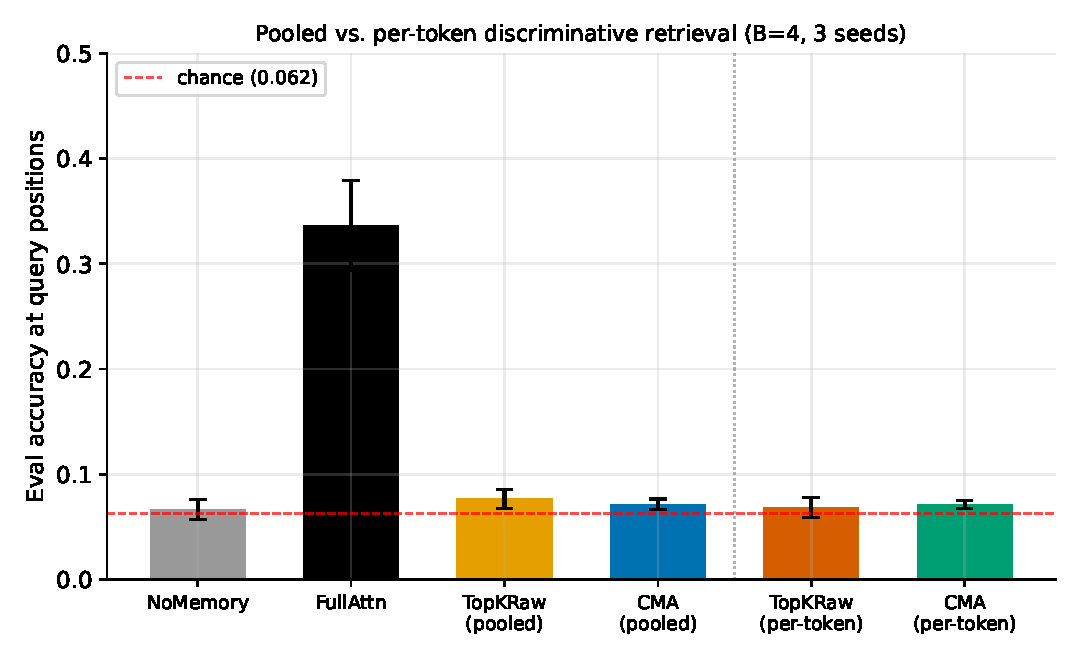
\includegraphics[width=0.85\linewidth]{figures/fig_pertoken_bar.pdf}
\caption{All four bounded-memory conditions, pooled and per-token retrieval, at $B{=}4$. Fixing
the retrieval-selection mechanism to be genuinely query-conditioned does not move any of them off
of chance.}
\label{fig:pertoken-bar}
\end{figure}

\paragraph{Where this leaves us.} Two candidate explanations for Observation 1 are now ruled out
with direct evidence: collapse-to-null (Diagnostic A, and its per-token-corrected re-run), and
vacuous chunk-level selection (Diagnostic B, first pass, corrected and then re-tested properly).
The most parsimonious explanation we have left is more mundane than either: the cross-attention
module's content-matching circuit itself --- learning, from a random initialization, to route each
query position's $Q$ toward the $K$ of the memory item that actually contains its answer --- may
simply not have been learned within 1300 steps, independent of how memory is organized or how
finely retrieval selection is conditioned on the query. This would be a cross-attention analogue of
the induction-head bootstrapping problem in Section~\ref{sec:calibration}, except harder: an
induction head can fall onto a simple, position-independent ``attend one step back'' pattern, while
matching a query token's content against the content of an arbitrary, previously-written memory
item has no comparably simple pattern to fall onto from initialization. We want to be explicit that
we have \emph{not} confirmed this: it is the leading remaining hypothesis by elimination, not a
third diagnostic with its own direct measurement, and we did not have compute budget left in this
study to test it further (Section~\ref{sec:limitations}).

\subsection{Secondary budget sweep ($B \in \{8, 16\}$, single seed)}
\label{sec:results-sweep}

Table~\ref{tab:sweep} and Figure~\ref{fig:budget-sweep} extend TopKRaw and CMA to $B{=}8$ (exactly
enough token-equivalent slots for all four pairs) and $B{=}16$ ($2\times$ headroom), single seed,
explicitly illustrative rather than a significance claim (Section~\ref{sec:setup}). Both methods
stay pinned to the same value across all three budgets and remain indistinguishable from
NoMemory's seed-0 accuracy. As Section~\ref{sec:results-diagnosis} discusses, we do not attribute
this flatness to memory-selection granularity: the same flat pattern persists in the follow-up
sweep under genuinely discriminative per-token retrieval (Table~\ref{tab:pertoken}), so budget and
retrieval granularity can both be ruled out as the limiting factor, leaving the cross-attention
content-matching circuit itself as the leading remaining explanation.

\begin{table}[H]
\centering
\small
\begin{tabular}{lccc}
\toprule
Condition & $B{=}4$ & $B{=}8$ & $B{=}16$ \\
\midrule
TopKRaw & 0.0674 & 0.0674 & 0.0674 \\
CMA & 0.0674 & 0.0674 & 0.0674 \\
\bottomrule
\end{tabular}
\caption{Single-seed (seed 0) illustrative budget sweep. All six values (both methods, all three
budgets) agree exactly with each other and with NoMemory's seed-0 accuracy to the precision of our
256-sequence, 4-query-per-sequence (1024-prediction) evaluation batch.}
\label{tab:sweep}
\end{table}

\begin{figure}[H]
\centering
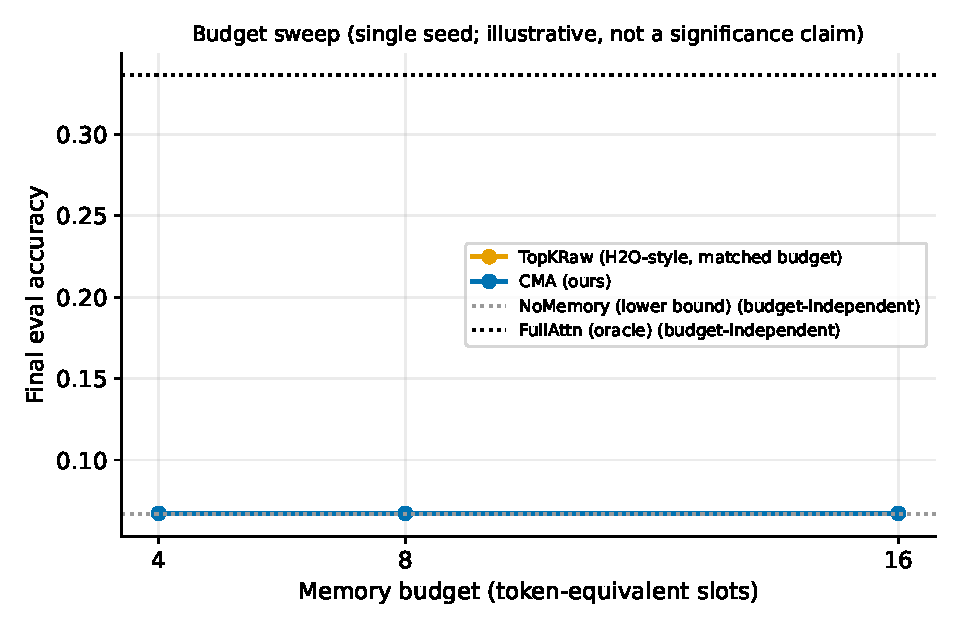
\includegraphics[width=0.66\linewidth]{figures/fig_budget_sweep.pdf}
\caption{Budget sweep, single seed. TopKRaw and CMA overlap completely across the full budget
range tested and track NoMemory rather than approaching FullAttn.}
\label{fig:budget-sweep}
\end{figure}

\subsection{A third candidate explanation, also ruled out: task difficulty}
\label{sec:results-easytask}

Section~\ref{sec:results-diagnosis} ruled out two mechanisms internal to the memory branch itself
(collapse to null, vacuous selection) but left one confound untouched: our task
(Section~\ref{sec:setup}) requires disambiguating among $P{=}4$ candidates drawn from a
16-symbol key vocabulary, with the query block only about 66 positions past the latest position a
pair could occupy in the worst case. If this was simply too hard a discrimination problem for a
randomly-initialized cross-attention circuit to get any traction on within 1300 steps, we would
expect exactly the flat pattern we observed, independent of whether retrieval selection is pooled
or per-token and independent of memory organization --- making task difficulty, not memory
architecture, the actual limiting factor. We test this directly rather than assume it.

\paragraph{A substantially easier, still purely content-matching task.} We lower $P$ from 4 to 2
pairs, shrink the key and value vocabularies from 16 to 8 symbols each, and lower
\texttt{insert\_region\_frac} from 0.6 to 0.4, which shrinks the window pairs can be inserted into
(positions 0--76 rather than 0--115) while the query block --- now only 2
\texttt{(QUERY, key, value)} triples instead of 4, so it starts later, at position 187 rather than
181 --- moves slightly later; combined, the worst-case gap between the end of the insertion
window and the start of the query block grows from 66 to 111 positions. We deliberately do
\emph{not} introduce any recency or overwrite structure (e.g., the same key written twice with the
query needing the more recent value): that variant admits a strictly easier fallback strategy,
``prefer the most recently written match,'' which does not require content-based key matching at
all and would not isolate the mechanism we are testing. Every other hyperparameter, and both
retrieval mechanisms (\textsc{TopKRaw-PT}, \textsc{CMA-PT}), are unchanged from
Section~\ref{sec:results-diagnosis}. Table~\ref{tab:easytask} and Figure~\ref{fig:easytask-bar}
show the result; raw per-seed values are in Table~\ref{tab:easytask-raw}, reported in full for the
same reason as Table~\ref{tab:primary-raw}.

\begin{table}[H]
\centering
\small
\begin{tabular}{lrrrr}
\toprule
Condition & Params & Eval accuracy (mean $\pm$ std) & Eval loss (mean) & $n$ seeds \\
\midrule
NoMemory (lower bound) & 105{,}984 & $0.1224 \pm 0.0030$ & 2.082 & 3 \\
FullAttn (oracle) & 105{,}984 & $0.6686 \pm 0.0386$ & 0.604 & 3 \\
TopKRaw-PT ($B{=}4$) & 139{,}136 & $0.1243 \pm 0.0060$ & 2.081 & 3 \\
CMA-PT ($B{=}4$) & 139{,}136 & $0.1178 \pm 0.0060$ & 2.080 & 3 \\
\bottomrule
\end{tabular}
\caption{Simplified-task comparison, $B{=}4$, 3 seeds. Chance-level accuracy is $1/8{=}0.125$
(smaller value vocabulary than the primary task's $1/16$, so these numbers are not directly
comparable in absolute terms to Table~\ref{tab:primary}; the comparison that matters is each
condition against this task's own chance level and against FullAttn on this same task).
Chance-level loss is $\ln 8 \approx 2.079$.}
\label{tab:easytask}
\end{table}

\begin{table}[H]
\centering
\small
\begin{tabular}{lccc}
\toprule
Condition & seed 0 & seed 1 & seed 2 \\
\midrule
NoMemory & 0.1191 & 0.1250 & 0.1230 \\
FullAttn & 0.6758 & 0.6270 & 0.7031 \\
TopKRaw-PT ($B{=}4$) & 0.1191 & 0.1309 & 0.1230 \\
CMA-PT ($B{=}4$) & 0.1191 & 0.1113 & 0.1230 \\
\bottomrule
\end{tabular}
\caption{Raw per-seed final evaluation accuracy underlying Table~\ref{tab:easytask}, reported in
full for the same reason as Table~\ref{tab:primary-raw}.}
\label{tab:easytask-raw}
\end{table}

\begin{figure}[H]
\centering
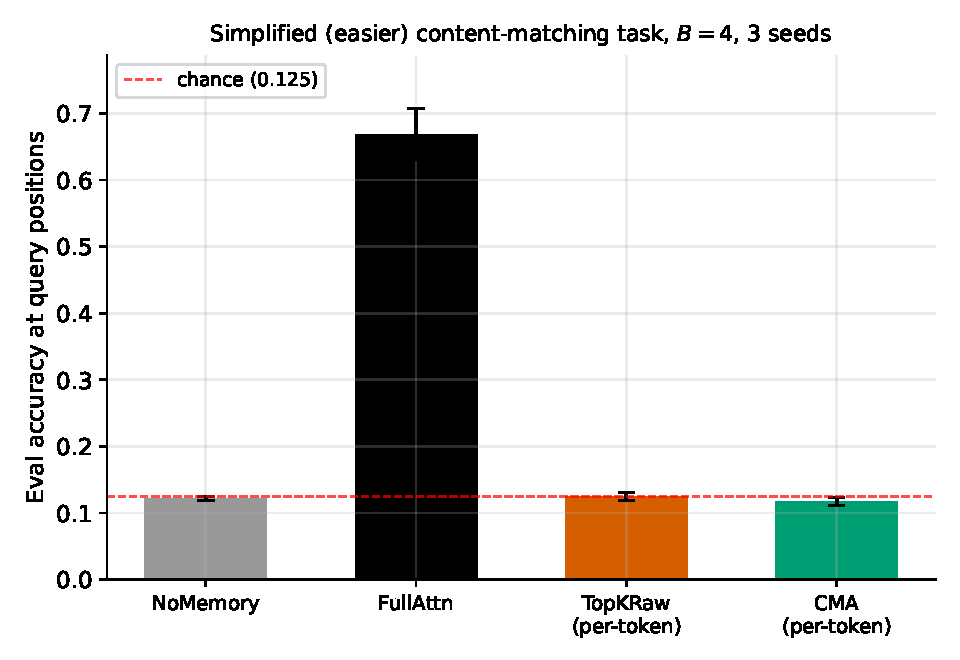
\includegraphics[width=0.62\linewidth]{figures/fig_easytask_bar.pdf}
\caption{Simplified-task comparison at $B{=}4$, 3-seed mean with standard-deviation error bars.
FullAttn separates sharply from chance; TopKRaw-PT and CMA-PT do not, and remain statistically
indistinguishable from each other and from NoMemory.}
\label{fig:easytask-bar}
\end{figure}

\paragraph{FullAttn confirms the task got easier; the bounded-memory methods do not move.}
FullAttn's accuracy nearly doubles relative to the primary task, from $0.336$
(Table~\ref{tab:primary}) to $0.669$ here, confirming the simplification worked: the underlying
recall problem is both learnable and substantially easier within the same 1300-step budget.
TopKRaw-PT and CMA-PT, however, are unchanged in kind: both remain within about one standard
deviation of this task's own chance level ($0.125$) and of each other. CMA-PT's mean
($0.1178$) is nominally \emph{below} TopKRaw-PT's ($0.1243$), a gap of $-0.0065$ --- if anything
the wrong sign for CMA, and well inside the noise given both standard deviations are $0.0060$. A
single-seed reference sweep to $B{=}8$ shows the same pattern: TopKRaw-PT and CMA-PT both score
exactly $0.1191$, identical to each other and to their own $B{=}4$, seed-0 values. Task difficulty
is therefore not the limiting factor: the discriminative signal FullAttn exploits is present and
learnable in this step budget, but neither bounded-memory method's retrieval pathway benefits from
it.

\paragraph{An exact-precision observation, and what we could and could not confirm about it.}
At seed 0, TopKRaw-PT ($B{=}4$), TopKRaw-PT ($B{=}8$), and CMA-PT ($B{=}8$) produce
\emph{bit-identical} evaluation accuracy at all thirteen checkpoints across the full 1300-step
run, not merely at the final one, and match NoMemory's seed-0 curve for the first five checkpoints
before diverging from it at step 600 onward. This is a stronger and more specific pattern than
Observation 1 in Section~\ref{sec:results-diagnosis} (final-value agreement only); we investigated
it rather than let it pass as a curiosity. Two things about it are directly verified. First,
neither memory bank class (\texttt{ClusterMemoryBank}, \texttt{RawTopKMemoryBank}) registers any
\texttt{nn.Parameter}; all memory content lives in plain tensors allocated in \texttt{reset()}.
Combined with the null fallback slot being a zero-initialized parameter (Section~\ref{sec:method}),
this means the learnable parameters of a TopKRaw-PT and a CMA-PT model, or of the same
architecture at different budgets, are initialized \emph{bit-identically} under the same random
seed --- which we confirmed directly by comparing \texttt{state\_dict()} tensors across
conditions rather than inferring it from the code alone. Second, we reran the null-attention-weight
diagnostic (Table~\ref{tab:null-attn}) under this task's hyperparameters
(Table~\ref{tab:null-attn-easytask}): the mean weight on the null fallback slot stabilizes around
$0.48$--$0.52$ for both mechanisms, the same order of magnitude as the primary task and, again, far
short of $1.0$ --- so collapse-to-null is not the explanation here either. What we did
\emph{not} verify directly is why bit-identical initialization and comparable, non-saturated null
weights produce bit-identical \emph{decisions}: our working explanation is that, this early in
training, the memory content's contribution to each query position's prediction is real (the null
weight is only $\approx$half) but not yet large enough, relative to the shared,
identically-initialized backbone's contribution, to flip the arg-max decision at any of the 512
evaluation queries across thirteen consecutive checkpoints and three different bounded-memory
configurations. This reading is consistent with, and does not contradict, our leading hypothesis
below; it is a plausible interpretation of already-verified facts, not a claim we tested with its
own diagnostic (e.g., by comparing logits rather than arg-max decisions), and we report it at that
lower confidence level explicitly rather than presenting it as confirmed.

\begin{table}[H]
\centering
\small
\begin{tabular}{lrrrr}
\toprule
Condition & step 1 & step 400 & step 800 & step 1300 \\
\midrule
TopKRaw-PT ($B{=}4$) & 0.441 & 0.503 & 0.516 & 0.516 \\
CMA-PT ($B{=}4$) & 0.441 & 0.480 & 0.503 & 0.490 \\
\bottomrule
\end{tabular}
\caption{Mean null-slot attention weight under this section's (easier-task) hyperparameters,
single seed, separate diagnostic run (same recipe as Table~\ref{tab:null-attn}, not a
continuation of the exact runs behind Table~\ref{tab:easytask}, since this diagnostic's
evaluation schedule samples an additional checkpoint at step 1 and therefore consumes the shared
evaluation-data generator on a different cadence). Stabilizes around $0.48$--$0.52$, the same
order of magnitude as the harder task's $0.28$--$0.44$ (Table~\ref{tab:null-attn}) and, again, far
from the $1.0$ that would indicate collapse to the fallback slot.}
\label{tab:null-attn-easytask}
\end{table}

\paragraph{Where this leaves us.} Three specific candidate explanations for the null result are
now ruled out by direct evidence: collapse to the null fallback slot (Table~\ref{tab:null-attn}),
vacuous query-independent retrieval selection (Section~\ref{sec:results-diagnosis}), and task
difficulty (this section, via a task on which FullAttn nearly doubles its accuracy while
TopKRaw-PT and CMA-PT do not move at all). Each was ruled out by a direct measurement targeting
that specific mechanism, not by assumption or by elimination alone. What remains is the same
leading hypothesis Section~\ref{sec:results-diagnosis} identified: the memory cross-attention's
content-matching circuit itself may simply need more training than we gave it, independent of
memory organization, retrieval granularity, or task difficulty. We did not test this directly, and
Section~\ref{sec:limitations} explains why we chose not to.

\subsection{Summary}
The narrow empirical question this paper set out to ask --- at equal memory budget, does
clustering organize memory better than raw top-$B$ token retention? --- is not answered by these
experiments, in either direction, under either retrieval mechanism, or on either task difficulty,
that we tried. Both methods are indistinguishable from a no-memory baseline and from each other at
every budget we tried, with pooled-chunk retrieval, again with genuinely discriminative per-token
retrieval (Section~\ref{sec:results-diagnosis}), and again on a substantially easier version of
the same task on which a full-attention oracle nearly doubles its accuracy
(Section~\ref{sec:results-easytask}). Rather than stop at an unexplained null result, or at our
first (incorrect) explanation for it, we used direct measurement and two corrected or redesigned
follow-up experiments to rule out three specific candidate causes --- collapse to the null
fallback slot, vacuous (query-independent) memory selection, and task difficulty --- leaving the
cross-attention content-matching circuit's own trainability as the most likely remaining
bottleneck, not yet confirmed by a direct test of its own, and one we chose not to pursue further
in this study (Section~\ref{sec:limitations}).

\section{Discussion and Limitations}
\label{sec:limitations}

We list limitations in order of how much we think they should temper the reader's confidence in
our conclusions, rather than in the order the topics were introduced.

\paragraph{The central comparison is inconclusive; we were wrong once while investigating why, and
we kept investigating twice more after correcting that.} Section~\ref{sec:results} shows that
neither TopKRaw nor CMA separates from a no-memory baseline, from each other, or across a
$4\times$ range of memory budget, despite direct measurement showing the memory cross-attention
assigns most of its weight to genuinely retrieved content rather than collapsing to its null
fallback (Table~\ref{tab:null-attn}). Our first explanation --- that a chunk-pooled
retrieval-selection query could not distinguish the multiple queries our task places in one chunk
--- turned out, on closer reading of our own \texttt{retrieve()} code, to describe a mechanism
(candidate selection) that our experimental configuration had already made a no-op for an
unrelated reason ($k_{\text{sim}}$ was set equal to full capacity, so top-$k$ selection selected
everything regardless of the query). We implemented and unit-tested a corrected, genuinely
query-conditioned retrieval mechanism, reran the full primary comparison and budget sweep under it,
and found the same null result (Section~\ref{sec:results-diagnosis}, Table~\ref{tab:pertoken}):
CMA still does not separate from TopKRaw. Suspecting the task itself might be too hard for the
mechanism to get traction on regardless of retrieval fidelity, we redesigned it to be substantially
easier while keeping it a pure content-matching problem, confirmed with a full-attention oracle
that it is in fact easier and learnable in our step budget, and found the same null result a third
time (Section~\ref{sec:results-easytask}, Table~\ref{tab:easytask}). Three specific candidate
explanations are now ruled out by direct evidence, each targeted at that explanation specifically
rather than inferred by elimination; the one hypothesis we have not ruled out or confirmed ---
that the cross-attention content-matching circuit itself has not been learned within our step
budget, regardless of memory organization, retrieval granularity, or task difficulty --- is not
yet tested by a diagnostic of its own, and we explain below why we chose not to pursue that test
in this study rather than treat the omission as an oversight. Given all of this, this paper's
central empirical question (does clustering beat raw retention at equal budget?) remains formally
open, not answered in either direction; what we report as this paper's actual result is the method
synthesis, the tested implementation, and a diagnostic process that caught and corrected its own
first mistake, then twice more ruled out a specific plausible confound with a targeted experiment
rather than stopping at an unexplained null --- which is what we deliver here instead of either an
unexplained null result, an uncorrected wrong explanation, or a fourth round chosen mainly to keep
looking for significance.

\paragraph{No real-language-model validation.} Everything in Section~\ref{sec:results} is on a
synthetic recall task with, at most, a 96-symbol vocabulary and a two-layer, $d{=}64$ model. This
isolates the mechanism we care about (does clustering preserve enough information under a tight
token budget) from confounds that a real corpus would introduce, but it is not evidence about
perplexity, downstream task accuracy, or behavior at realistic model and context scale. We see
this as the single most important piece of follow-up work, and we are specific about what it would
take rather than leaving it as a vague ``more compute needed'': validating on a real or
semi-real long-context NLP task (for example, long-document question answering or multi-session
dialogue, per the survey in Section~\ref{sec:related}) with minimal fine-tuning of a small
pretrained backbone (roughly 100M--1B parameters, not a from-scratch toy transformer) would need
one GPU with on the order of 16--24GB of memory --- a single consumer or entry-level cloud card
(e.g., an RTX~3090/4090 or A10-class instance), not a cluster --- which is a deliberately modest
target consistent with this paper's small-scale approach throughout, not a claim that a larger
validation is unnecessary. We do not have that available in this study and report it as untested
rather than simulate it with a smaller proxy that would not actually answer the question.

\paragraph{Compute-constrained statistical power.} Our environment had two CPU cores and no GPU.
The primary comparison uses 3 seeds; the budget-sweep beyond $B{=}4$ uses a single seed per
condition and is explicitly illustrative rather than a claim with error bars. Three seeds is
enough to report a mean and range but not enough for strong significance claims; we report both
so readers can judge for themselves rather than us asserting significance we cannot support. We
did not scale the primary comparison up to more seeds after Section~\ref{sec:results-easytask}'s
third null result: with the CMA-minus-TopKRaw gap already near zero and, if anything,
sign-reversed ($-0.0065$, both standard deviations $0.0060$), more seeds would sharpen the
confidence interval around that small, wrong-signed gap rather than plausibly turn it into a
meaningfully positive one --- an effect-size problem, not a statistical-power problem, so more
seeds on the same task and step budget is not the experiment we judged worth running next.

\paragraph{Training budget may leave the task under-converged --- a related but distinct question
we chose not to chase.} Section~\ref{sec:calibration} shows FullAttn still improving, not
plateaued, at step 1300. The relative ordering between conditions at a fixed, shared, and modest
step budget is a meaningful comparison of \emph{sample efficiency} under our specific optimizer
schedule, but it is not the same claim as ``condition X's asymptotic ceiling is higher than
condition Y's''; a longer training budget could change whether TopKRaw-PT or CMA-PT ever separate
from chance at all, which is a different question from whether more \emph{seeds} at our current
step budget would (Compute-constrained statistical power, above). If the memory cross-attention's
content-matching circuit simply needs more steps to bootstrap than self-attention's induction heads
do, a substantially longer run (we would guess on the order of $5{,}000$+ steps, several times our
budget) is the experiment that would tell us, and we did not run it. This is a deliberate scope
decision, not a claim that we tested it and it would not help: extending training speaks to
training dynamics in this synthetic setup, which is one step removed from this paper's actual
question (does clustering organize memory better than raw retention, once both can use their
memory at all?), and we judged the three-round exclusion chain we already have --- collapse to
null, vacuous selection, and task difficulty, all ruled out --- to be a more useful contribution
to report now than a fourth round chasing a question this paper was not originally built to answer.
We leave it, explicitly, as the concrete next experiment for anyone who wants to pursue it.

\paragraph{Cluster assignment is not end-to-end optimized in these experiments.} CMA's optional
straight-through/commitment-loss training path (Section~\ref{sec:method}, M2) is implemented and
unit-tested but was \emph{not} used in the reported experiments: the memory write is a
stop-gradient operation, so the backbone receives no gradient signal encouraging it to produce
more ``clusterable'' hidden states at write time --- only the read path is trained. This matches
how Memorizing Transformers and EM-LLM also treat their memories, but it means our results are a
lower bound on what CMA could do if the write path were trained; we did not have compute budget
remaining to test the alternative.

\paragraph{The importance-score proxy is crude.} Both CMA's exemplar selection and the TopKRaw
baseline rank tokens by hidden-state $\ell_2$ norm, which is only a proxy for how useful a token
actually is to retrieve later. We use the identical proxy in both conditions specifically so
that whatever bias it introduces should apply symmetrically, but a real attention-weight-based
score (as ClusterAttn or H2O use, and as our reference implementation supports) might change the
absolute numbers for both methods.

\paragraph{The merge operation is an approximation.} M2's cluster merge uses a count-weighted
linear combination of centroids, renormalized, as a cheap stand-in for a true spherical mean; we
did not evaluate how much this costs relative to an iterative spherical $k$-means-style update.

\paragraph{Hyperparameters were calibrated, not tuned.} The learning rate schedule, chunk size,
and merge threshold were fixed during a short calibration pass (Section~\ref{sec:calibration})
aimed at making the task learnable at all, not at optimizing CMA's or the baseline's accuracy;
we did not run a hyperparameter sweep for either bounded-memory method, so the comparison in
Section~\ref{sec:results} should be read as ``under one reasonable, shared setting,'' not as
each method's best case. The same applies to the follow-up experiment's $k_{\text{sim}} = $
half of capacity (Section~\ref{sec:results-diagnosis}): we picked ``half'' as a reasonable value
that makes selection non-vacuous without trying alternatives such as a quarter or three-quarters
of capacity.

\paragraph{Search scope for related work.} Section~\ref{sec:related}'s claim that we did not
find prior work combining bounded-capacity clustering with online merge/eviction reflects the
scope and time budget of one literature search conducted in July 2026, not a systematic review;
Table~\ref{tab:provenance}'s ``new here'' column should be read with that caveat.

\section{Conclusion}

We assembled Clustered Memory Augmentation from a mix of directly adapted components (EM-LLM's
segmentation and dual-buffer retrieval, ClusterAttn's and H2O's importance-based token scoring,
HMT's plug-in integration) and one combination we believe is new in this context: pairing
DP-means-style dynamic cluster creation with VQ-VAE-style EMA updates and stop-gradient training
to get a memory whose cluster count is provably bounded and can merge and evict as a stream runs
indefinitely (Table~\ref{tab:provenance}). We built and unit-tested a reference implementation,
then asked a narrow, falsifiable empirical question on a synthetic long-range recall task: at
equal memory budget, does clustering organize memory better than keeping the raw highest-scoring
tokens? Section~\ref{sec:results} reports what we found under a fixed, modest compute budget, in
three rounds. At our primary tight budget, neither method separates from a no-memory baseline or
from each other, and this null pattern persists exactly across a further $4\times$ single-seed
budget sweep. Rather than leave that as an unexplained negative result, we instrumented the model
directly and ruled out the simplest explanation (the memory branch collapsing to ignore retrieved
content). Our next explanation --- that a chunk-pooled retrieval-selection query could not
distinguish the multiple queries our task packs into one chunk --- was itself wrong, in a specific
and checkable way we found by re-reading our own retrieval code: the experimental configuration
had already made candidate selection query-independent for an unrelated reason, so pooled versus
per-token could not have mattered. We implemented, unit-tested, and ran a corrected version with
retrieval selection that is genuinely conditioned on a per-token query, and obtained the same null
result again (Section~\ref{sec:results-diagnosis}). Suspecting the task's difficulty itself might
be the confound, we then redesigned it to be substantially easier while keeping it a pure
content-matching problem --- confirmed easier and learnable in our step budget by a full-attention
oracle whose accuracy nearly doubles --- and obtained the same null result a third time
(Section~\ref{sec:results-easytask}). Three specific candidate explanations are consequently ruled
out by direct evidence, each by a measurement aimed at that explanation and not by elimination
alone; what remains is the more mundane possibility that the memory cross-attention's
content-matching circuit has not been learned within our step budget, independent of memory
organization, retrieval granularity, or task difficulty, which we have not tested directly.

We stop here by deliberate choice, not because we ran out of things to try. Two different
``run more'' options were available to us --- more seeds on the comparison we already have, or a
substantially longer training run --- and we think it is worth being precise about why we did
neither. More seeds would sharpen the confidence interval around a gap that is already small and,
if anything, sign-reversed against CMA ($-0.0065$); that is an effect-size problem, and more
seeds do not fix an effect-size problem, they just measure it more precisely. A substantially
longer training run is a genuinely different experiment --- it speaks to whether the
content-matching circuit can bootstrap at all given enough steps, not to whether clustering beats
raw retention once it can --- and we see it as a legitimate next experiment for anyone who wants
to run it, not as something we ruled out; we simply judged three targeted, direct-evidence
exclusions to be a more complete and useful thing to hand off than a fourth round chasing a
question this paper was not originally built to answer. We see the result of this study as the
method synthesis, the tested implementation, and the exclusion chain itself --- three specific,
independently plausible explanations for a stubborn null result, each ruled out by a measurement
built for that explanation rather than assumed away, including one case where our own first
explanation was wrong and we said so before moving on. What we do not offer is a resolution of the
question we set out to ask: whether clustering organizes bounded memory better than raw retention
remains open, and the one hypothesis that could still explain our null result --- that the circuit
needs training we did not give it --- is left as a concrete, named, and deliberately untested
next step, not as an oversight or a resource shortfall.

\section*{Acknowledgments}
This work's method design, implementation, and experiments were carried out in collaboration
with Claude (Anthropic). See the footnote on page~1 for a full disclosure statement.

\begin{thebibliography}{99}

\bibitem[Arora et al., 2024]{arora2024zoology} S.~Arora, S.~Eyuboglu, A.~Timalsina, et al.
Zoology: Measuring and Improving Recall in Efficient Language Models. \emph{ICLR}, 2024.
\url{https://arxiv.org/abs/2312.04927}

\bibitem[ClusterAttn, 2025]{clusterattn2025} ClusterAttn: KV Cache Compression under Intrinsic
Attention Clustering. \emph{ACL}, 2025. \url{https://aclanthology.org/2025.acl-long.703/}

\bibitem[Dai et al., 2019]{dai2019transformerxl} Z.~Dai, Z.~Yang, Y.~Yang, et al. Transformer-XL:
Attentive Language Models Beyond a Fixed-Length Context. 2019.
\url{https://arxiv.org/abs/1901.02860}

\bibitem[DP-means, 2012]{dpmeans2012} B.~Kulis, M.~I.~Jordan. Revisiting $k$-means: New
Algorithms via Bayesian Nonparametrics. \emph{ICML}, 2012.
\url{https://arxiv.org/abs/1111.0352}

\bibitem[EM-LLM, 2025]{emllm2025} Human-inspired Episodic Memory for Infinite Context LLMs
(EM-LLM). \emph{ICLR}, 2025. \url{https://arxiv.org/abs/2407.09450}

\bibitem[He et al., 2025]{he2025hmt} HMT: Hierarchical Memory Transformer for Efficient Long
Context Language Processing. \emph{NAACL}, 2025.
\url{https://aclanthology.org/2025.naacl-long.410/}

\bibitem[Khandelwal et al., 2020]{khandelwal2020knnlm} U.~Khandelwal, O.~Levy, D.~Jurafsky, et al.
Generalization through Memorization: Nearest Neighbor Language Models. \emph{ICLR}, 2020.
\url{https://arxiv.org/abs/1911.00172}

\bibitem[Kitaev et al., 2020]{kitaev2020reformer} N.~Kitaev, {\L}.~Kaiser, A.~Levskaya. Reformer:
The Efficient Transformer. \emph{ICLR}, 2020. \url{https://arxiv.org/abs/2001.04451}

\bibitem[Lample et al., 2019]{lample2019memory} G.~Lample, A.~Sablayrolles, M.~Ranzato, et al.
Large Memory Layers with Product Keys. \emph{NeurIPS}, 2019.
\url{https://arxiv.org/abs/1907.05242}

\bibitem[Meta, 2024]{meta2024memorylayers} Memory Layers at Scale. 2024.
\url{https://arxiv.org/abs/2412.09764}

\bibitem[MoSA, 2025]{mosa2025} Mixture of Sparse Attention: Content-Based Learnable Sparse
Attention via Expert-Choice Routing. 2025. \url{https://arxiv.org/abs/2505.00315}

\bibitem[Olsson et al., 2022]{olsson2022induction} C.~Olsson, N.~Elhage, N.~Nanda, et al.
In-context Learning and Induction Heads. \emph{Transformer Circuits Thread}, 2022.
\url{https://arxiv.org/abs/2209.11895}

\bibitem[Rae et al., 2020]{rae2020compressive} J.~W.~Rae, A.~Potapenko, S.~M.~Jayakumar, et al.
Compressive Transformers for Long-Range Sequence Modelling. \emph{ICLR}, 2020.
\url{https://arxiv.org/abs/1911.05507}

\bibitem[Survey, 2025]{survey2025} Memory-Augmented Transformers: A Systematic Review from
Neuroscience Principles to Technical Solutions. 2025. \url{https://arxiv.org/abs/2508.10824}

\bibitem[Roy et al., 2021]{roy2021routing} A.~Roy, M.~Saffar, A.~Vaswani, D.~Grangier. Efficient
Content-Based Sparse Attention with Routing Transformers. \emph{TACL}, 2021.
\url{https://arxiv.org/abs/2003.05997}

\bibitem[Titans, 2025]{titans2025} A.~Behrouz, et al. Titans: Learning to Memorize at Test Time.
\emph{Google Research}, 2025. \url{https://arxiv.org/abs/2501.00663}

\bibitem[van den Oord et al., 2017]{vqvae2017} A.~van den Oord, O.~Vinyals, K.~Kavukcuoglu.
Neural Discrete Representation Learning. \emph{NeurIPS}, 2017.
\url{https://arxiv.org/abs/1711.00937}

\bibitem[Wang et al., 2020]{wang2020clusterformer} S.~Wang, L.~Zhou, Z.~Gan, et al. Cluster-Former:
Clustering-based Sparse Transformer for Long-Range Dependency Encoding. 2020.
\url{https://arxiv.org/abs/2009.06097}

\bibitem[Wu et al., 2022]{wu2022memorizing} Y.~Wu, M.~N.~Rabe, D.~Hutchins, C.~Szegedy. Memorizing
Transformers. \emph{ICLR}, 2022. \url{https://arxiv.org/abs/2203.08913}

\bibitem[Xiao et al., 2024]{xiao2024streaming} G.~Xiao, Y.~Tian, B.~Chen, et al. Efficient
Streaming Language Models with Attention Sinks. \emph{ICLR}, 2024.
\url{https://arxiv.org/abs/2309.17453}

\bibitem[Zhang et al., 2023]{zhang2023h2o} Z.~Zhang, Y.~Sheng, T.~Zhou, et al. H$_2$O:
Heavy-Hitter Oracle for Efficient Generative Inference of Large Language Models. \emph{NeurIPS},
2023. \url{https://arxiv.org/abs/2306.14048}

\end{thebibliography}

\end{document}
